\chapter{Supporting Study: Road Logic \& CARLA (Nghiên cứu road logic và CARLA)}

Road logic và traffic là yêu cầu của hệ thống nhưng không thuộc về một reconstruction approach nào, nên có chương riêng.

\section{Tham khảo: NuRec kết hợp với CARLA như thế nào?}

Mục này giải thích cách NVIDIA nối NuRec với CARLA, dựa trên tài liệu chính thức và mã nguồn của CARLA\footnote{\url{https://carla.readthedocs.io/en/latest/nvidia_nurec/}; mã nguồn ở \texttt{PythonAPI/examples/nvidia/nurec}, nhánh \texttt{ue4-dev}, \url{https://github.com/carla-simulator/carla}}.
Nhóm có thể dùng ý tưởng này để tự triển khai cách nối tương tự cho các method khác.

NuRec và CARLA đảm nhận hai vai trò khác nhau nhưng bổ sung cho nhau:

\begin{table}[H]
  \centering
  \caption{Vai trò của từng thành phần}
  \begin{tabularx}{\linewidth}{>{\raggedright\arraybackslash}p{3cm} X}
    \toprule
    \textbf{Thành phần} & \textbf{Vai trò} \\
    \midrule
    NuRec & Tái dựng và render hình ảnh môi trường thực từ dữ liệu camera và LiDAR \\
    \addlinespace
    CARLA & Quản lý thế giới mô phỏng, trạng thái xe, các xe khác và tương tác khi chạy \\
    \addlinespace
    NuRec gRPC API & Giao diện để chương trình yêu cầu NuRec tạo ảnh từ vị trí camera được chỉ định \\
    \addlinespace
    Python script & Gọi cả hai bên, đồng bộ camera và thời gian \\
    \bottomrule
  \end{tabularx}
\end{table}

Nói đơn giản: CARLA quyết định điều gì đang xảy ra trong thế giới mô phỏng, còn NuRec làm cho thế giới đó trông giống môi trường thực được ghi hình.

\subsection{Vì sao cần kết hợp?}

Giả sử nhóm có dữ liệu quay từ một chiếc ô tô chạy trên đường ở Hà Nội, và muốn dùng dữ liệu đó để thử hệ thống ADAS.

\begin{figure}[H]
  \centering
  \begin{minipage}[t]{0.48\linewidth}
    \centering
    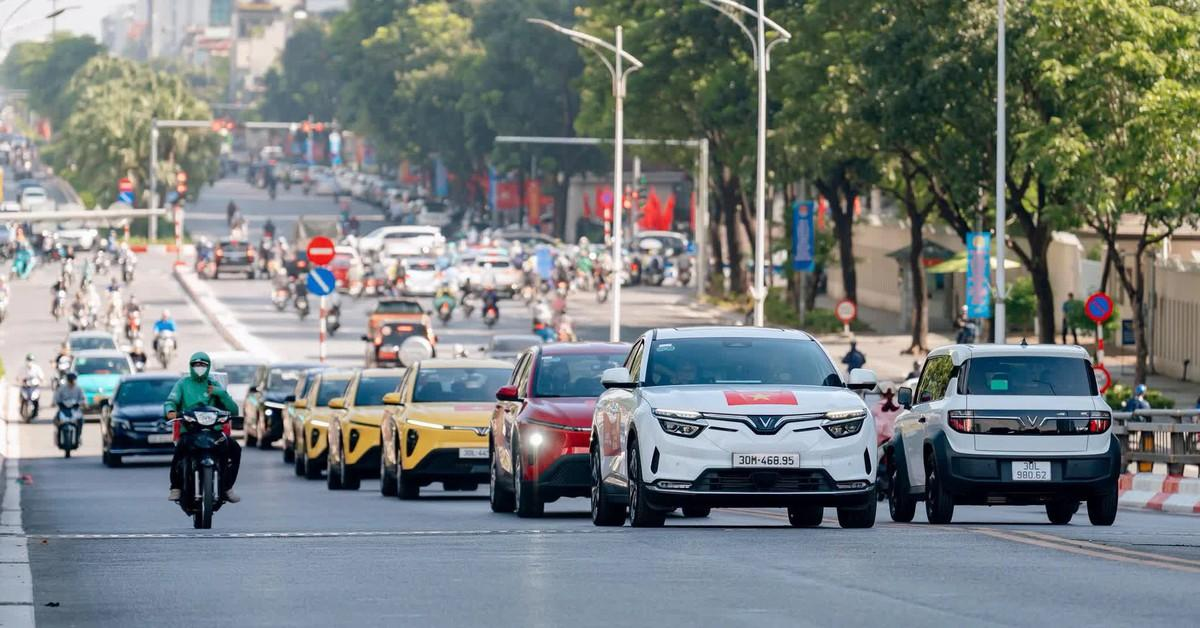
\includegraphics[width=\linewidth,height=4.2cm,keepaspectratio]{nurec-carla/real-driving-data.jpg}\\[3pt]
    \small Dữ liệu thực: camera ghi lại đường, xe và môi trường xung quanh (ảnh minh họa: Tuổi Trẻ Online)
  \end{minipage}\hfill
  \begin{minipage}[t]{0.48\linewidth}
    \centering
    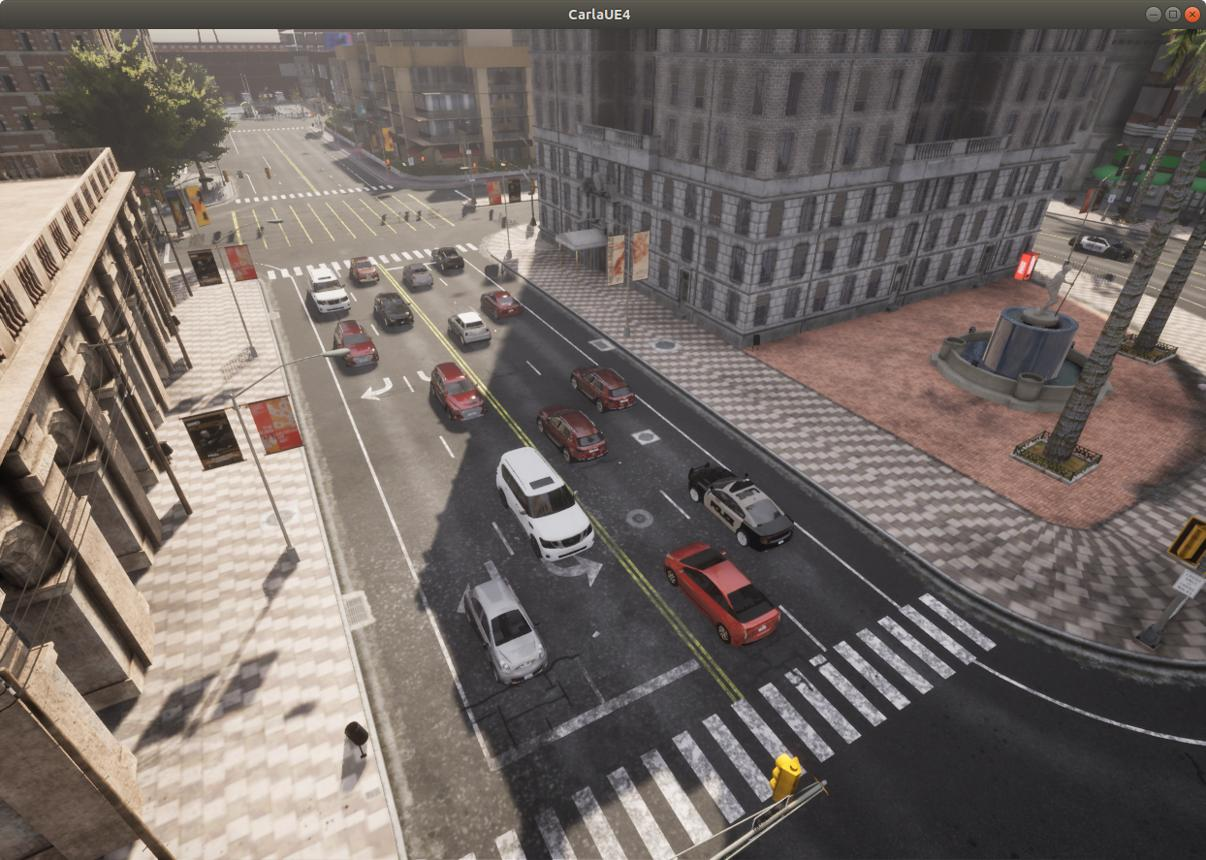
\includegraphics[width=\linewidth,height=4.2cm,keepaspectratio]{nurec-carla/carla-world.jpg}\\[3pt]
    \small Môi trường CARLA: xe và giao thông được quản lý trong thế giới ảo (ảnh: tài liệu CARLA)
  \end{minipage}
  \caption{Dữ liệu thực và môi trường CARLA}
\end{figure}

Ví dụ một bài kiểm thử:
\begin{enumerate}
  \item Xe tự lái chạy lại trên đoạn đường đã ghi hình.
  \item Một chiếc xe khác bất ngờ chuyển làn.
  \item Xe tự lái phải phát hiện nguy hiểm và phanh.
  \item Nhóm đổi tốc độ của xe cắt ngang và chạy lại bài kiểm thử.
  \item Hệ thống ghi nhận ADAS có phanh đúng lúc hay không.
\end{enumerate}

Nếu chỉ dùng video gốc thì không thể đổi vị trí camera hay tạo diễn biến mới.
Nếu chỉ dùng CARLA thì mô phỏng được giao thông, nhưng môi trường 3D không nhất thiết giống địa điểm thực.
Kết hợp hai bên cho phép có cả hình ảnh của nơi thật lẫn khả năng tương tác.

\subsection{NuRec làm những việc gì?}

NuRec có 2 công việc cần phân biệt rõ.

\textbf{Công việc A: Reconstruction (tái dựng).}
Đầu vào thường gồm camera, LiDAR, thông số hiệu chuẩn, vị trí xe theo thời gian và nhãn của vật thể chuyển động.
NuRec cần học được: mặt đường, tòa nhà, cây cối nằm ở đâu; môi trường trông thế nào từ nhiều góc; vật thể nào chuyển động; camera và vật thể ở đâu tại mỗi thời điểm.
Kết quả được đóng gói thành một USDZ scene, gồm mô tả scene, model đã train và các trajectory (quỹ đạo của đối tượng theo thời gian).

\begin{figure}[H]
  \centering
  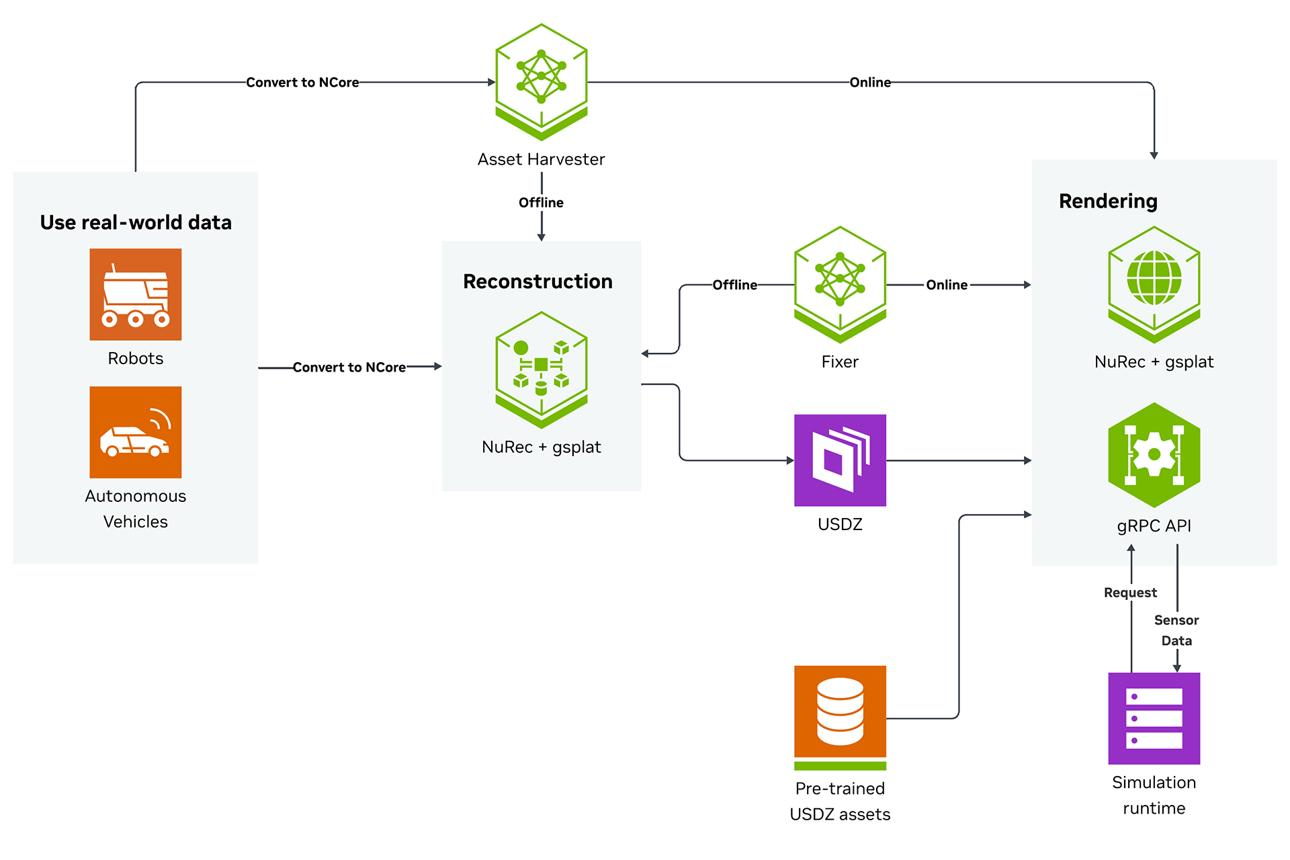
\includegraphics[width=0.85\linewidth]{nurec-carla/nurec-workflow.jpg}
  \caption{Luồng làm việc của NuRec (ảnh: NVIDIA Developer)}
\end{figure}

\textbf{Công việc B: Neural rendering (tạo ảnh).}
Đây là phần quan trọng khi kết hợp với CARLA.
Sau khi có scene, chương trình yêu cầu: quan sát cảnh này từ camera tại vị trí $(x, y, z)$, quay theo hướng $R$, ở thời điểm $t$.
NuRec tạo được ảnh từ góc nhìn đó, dù không có video thật quay đúng vị trí ấy. Kỹ thuật này gọi là novel view synthesis.

Ví dụ, xe ngoài đời chạy giữa làn, trong mô phỏng xe dịch sang trái 1 mét, NuRec có thể tạo góc nhìn mới tương ứng.
Khi camera đi quá xa vùng đã ghi nhận, các chi tiết có thể bị méo hoặc thiếu.

\subsection{Kiến trúc 3 thành phần}

Hệ thống gồm 3 thành phần chạy riêng biệt.
CARLA Server không tự gửi dữ liệu sang NuRec: Python script là phần gọi cả hai bên.

\begin{figure}[H]
  \centering
  \begin{tikzpicture}[
      box/.style={draw=accent, fill=blue!4, rounded corners=2pt, align=center,
                  text width=3.9cm, minimum height=2.5cm, font=\scriptsize\sffamily},
      result/.style={draw=accent, fill=blue!4, rounded corners=2pt, align=center,
                  text width=6cm, minimum height=0.8cm, font=\scriptsize\sffamily},
      flow/.style={<->, >={Stealth[length=2mm]}, thick, color=black!65},
      one/.style={-{Stealth[length=2mm]}, thick, color=black!65},
      lbl/.style={font=\tiny\sffamily, color=black!70}]
    \node[box] (carla) at (-5.4,0) {\textbf{CARLA Server}\\[2pt]Road map, world\\Ego vehicle\\Các xe khác\\Vật lý, thời gian mô phỏng};
    \node[box] (py) at (0,0) {\textbf{Python script}\\[2pt]Điều phối mô phỏng\\Gọi cả hai API\\Đồng bộ camera và thời gian};
    \node[box] (nr) at (5.4,0) {\textbf{NuRec Container}\\[2pt]Reconstructed scene\\Neural renderer\\Camera model};
    \node[result] (img) at (0,-2.3) {\textbf{Dữ liệu cảm biến mô phỏng}: ảnh camera do NuRec tạo};
    \draw[flow] (carla) -- node[lbl, above] {CARLA API} (py);
    \draw[flow] (py) -- node[lbl, above] {gRPC API} (nr);
    \draw[one] (py) -- (img);
  \end{tikzpicture}
  \caption{Kiến trúc NuRec + CARLA}
\end{figure}

\textbf{API} là giao diện để một chương trình yêu cầu chương trình khác làm việc.
Ví dụ, qua CARLA API, script lấy được trạng thái thế giới và vị trí xe:

\begin{lstlisting}[language=Python, numbers=none, caption={Đọc trạng thái qua CARLA API}]
world = client.get_world()
vehicle_pose = vehicle.get_transform()
\end{lstlisting}

\textbf{gRPC} là công nghệ gọi hàm từ xa giữa các chương trình.
Script gửi yêu cầu render đến NuRec Container và nhận lại ảnh.
Dưới đây là yêu cầu thật, rút gọn từ hàm \texttt{generate\_request} trong \texttt{nurec\_integration.py}:

\begin{lstlisting}[language=Python, numbers=none, texcl=true, caption={Yêu cầu render gửi đến NuRec (rút gọn từ mã nguồn CARLA)}]
RGBRenderRequest(
    scene_id=scene_id,
    resolution_h=int(camera_spec.resolution_h * scale),
    resolution_w=int(camera_spec.resolution_w * scale),
    camera_intrinsics=camera_spec,
    frame_start_us=timestamp,
    frame_end_us=timestamp + 1,      # hai giá trị phải khác nhau
    sensor_pose=PosePair(start_pose=pose, end_pose=pose),
    dynamic_objects=dynamic_objects, # vị trí các xe lấy từ CARLA
    image_format=ImageFormat.JPEG,
    image_quality=95,
)
\end{lstlisting}

Trong đó:
\begin{itemize}
  \item \texttt{scene\_id}: scene được chọn.
  \item \texttt{camera\_intrinsics}: thông số bên trong camera như tiêu cự, điểm chính và mô hình biến dạng.
  \item \texttt{sensor\_pose}: vị trí và hướng camera trong thế giới 3D.
  \item \texttt{frame\_start\_us}, \texttt{frame\_end\_us}: thời điểm cần render, tính bằng micro giây.
  \item \texttt{dynamic\_objects}: các vật thể chuyển động và vị trí của chúng.
\end{itemize}

\subsection{Một vòng mô phỏng}

Một vòng closed-loop đầy đủ diễn ra như sau. Thuật toán ADAS ở bước 4 không có sẵn trong ví dụ của CARLA, nhóm phải tự nối vào.

\begin{figure}[H]
  \centering
  \begin{tikzpicture}[
      box/.style={draw=accent, fill=blue!4, rounded corners=2pt, align=center,
                  text width=2.45cm, minimum height=1.25cm, font=\scriptsize\sffamily},
      flow/.style={-{Stealth[length=2mm]}, thick, color=black!65},
      lbl/.style={font=\tiny\sffamily, color=black!70}]
    \node[box] (a) at (0,0) {\textbf{1. CARLA}\\Cập nhật vị trí xe và đồng hồ};
    \node[box] (b) at (3.2,0) {\textbf{2. Python}\\Đọc vị trí camera và thời điểm};
    \node[box] (c) at (6.4,0) {\textbf{3. NuRec}\\Render ảnh camera};
    \node[box] (d) at (9.6,0) {\textbf{4. ADAS}\\Phát hiện, lên đường đi, ra lệnh};
    \node[box] (e) at (12.8,0) {\textbf{5. CARLA}\\Nhận lệnh ga, phanh, lái};
    \draw[flow] (a) -- (b);
    \draw[flow] (b) -- (c);
    \draw[flow] (c) -- (d);
    \draw[flow] (d) -- (e);
    \draw[flow] (e.south) -- ++(0,-0.5) -| node[lbl, pos=0.25, below] {bước mô phỏng tiếp theo} (a.south);
  \end{tikzpicture}
  \caption{Một vòng closed-loop}
\end{figure}

\subsection{Ví dụ của CARLA thực sự làm gì?}

File ví dụ tên là \texttt{example\_nurec\_replay\_save\_images.py}, và tài liệu CARLA gọi đây là replay.
Tuy nhiên, đọc mã nguồn cho thấy ví dụ này đã làm nhiều hơn replay thuần túy:

\begin{itemize}
  \item Ban đầu, xe ego được đặt lại theo quỹ đạo đã ghi bằng \texttt{set\_transform}, chưa bật vật lý.
  \item Sau 1 giây, script gọi \texttt{set\_ego\_simple\_trajectory\_following()}. Xe ego được bật vật lý và do bộ điều khiển \texttt{SimpleTrajectoryFollower} lái bằng lệnh ga, phanh, lái.
  \item Vị trí camera gửi cho NuRec được tính từ vị trí hiện tại của xe trong CARLA (\texttt{actor.get\_transform()}), không phải từ quỹ đạo đã ghi.
  \item Mã nguồn có sẵn \texttt{apply\_ego\_control(control)} để đưa lệnh lái từ bên ngoài vào xe.
\end{itemize}

Như vậy, phần ảnh đã đi theo xe trong CARLA. Phần còn thiếu là bộ điều khiển trong ví dụ chỉ bám theo quỹ đạo đã ghi và không dùng ảnh camera.
Muốn có closed-loop đúng nghĩa, cần thay bộ điều khiển đó bằng thuật toán nhận ảnh từ NuRec.

\begin{table}[H]
  \centering
  \caption{Replay, ví dụ của CARLA và closed-loop}
  \begin{tabularx}{\linewidth}{>{\raggedright\arraybackslash}p{2.9cm} X X X}
    \toprule
     & \textbf{Replay thuần} & \textbf{Ví dụ của CARLA} & \textbf{Closed-loop} \\
    \midrule
    Xe ego & Theo quỹ đạo ghi sẵn & Bám quỹ đạo ghi sẵn, có vật lý & Theo lệnh của ADAS \\
    \addlinespace
    Ảnh & Render theo vị trí replay & Render theo vị trí xe trong CARLA & Render theo vị trí xe trong CARLA \\
    \addlinespace
    Lệnh lái lấy từ & Không có & Bộ bám quỹ đạo & ADAS dựa trên ảnh \\
    \addlinespace
    Quyết định ảnh hưởng đến cảnh sau & Không & Có, nhưng không dựa trên ảnh & Có \\
    \bottomrule
  \end{tabularx}
\end{table}

\begin{warning}
Chạy được script replay không chứng minh đã có closed-loop ADAS.
Vẫn cần nối AD Stack và kiểm tra lệnh điều khiển thực sự tác động vào trạng thái CARLA.
\end{warning}

\subsection{NuRec có tự tạo road logic cho CARLA không?}

Không nên mặc định là có.
Một scene có thể chứa hình ảnh vạch kẻ làn và đèn giao thông rất thật, nhưng simulator chưa chắc hiểu được các thông tin đó.

\begin{table}[H]
  \centering
  \caption{Hình ảnh tái dựng khác với road logic}
  \begin{tabularx}{\linewidth}{>{\raggedright\arraybackslash}p{3cm} X X}
    \toprule
    \textbf{Thành phần} & \textbf{NuRec reconstruction} & \textbf{Road logic / CARLA} \\
    \midrule
    Vạch kẻ đường & Có thể tái dựng & Cần biết ranh giới và kết nối làn \\
    \addlinespace
    Đèn đỏ & Có thể render & Cần trạng thái và quy tắc điều khiển \\
    \addlinespace
    Mặt đường & Có lớp road geometry & Cần mặt đường lái được, hình học và vật lý phù hợp \\
    \addlinespace
    Xe đang chạy & Có thể tái dựng và chỉnh track & Cần hành vi và quỹ đạo đồng bộ với simulator \\
    \addlinespace
    Ngã tư & Có thể tái dựng cảnh & Cần kết nối làn và quy tắc ưu tiên \\
    \bottomrule
  \end{tabularx}
\end{table}

Tài liệu NVIDIA cho biết USDZ có thể chứa bản đồ OpenDRIVE nhưng không bắt buộc.
Tuy nhiên, script của CARLA đọc \texttt{map.xodr} từ USDZ và báo lỗi nếu không có.
CARLA dùng file này để tạo thế giới bằng \texttt{generate\_opendrive\_world}.
Vì vậy, muốn đi theo cách này, scene của nhóm phải có bản đồ OpenDRIVE khớp với cảnh tái dựng.

Ngoài ra, đổi vị trí hiển thị của một xe trong NuRec chưa có nghĩa xe đó có hành vi lái, logic tránh va chạm và trạng thái vật lý trong CARLA.

\subsection{Liên hệ với kiến trúc của nhóm}

Cách làm này khớp với 2 giai đoạn ở chương 2.
Giai đoạn offline chạy trước và thường tốn tính toán hơn. Giai đoạn online lặp lại ở từng bước mô phỏng.

\begin{figure}[H]
  \centering
  \begin{tikzpicture}[
      box/.style={draw=accent, fill=blue!4, rounded corners=2pt, align=center,
                  text width=2.6cm, minimum height=1cm, font=\scriptsize\sffamily},
      flow/.style={-{Stealth[length=2mm]}, thick, color=black!65},
      lbl/.style={font=\tiny\sffamily, color=black!70},
      stage/.style={font=\scriptsize\sffamily\bfseries, color=accent, anchor=west}]
    \node[stage] at (-1.4,1) {Offline: tái dựng};
    \node[box] (a) at (0,0) {Dữ liệu thật};
    \node[box] (b) at (3.6,0) {Chuẩn bị dữ liệu\\camera, LiDAR, pose, track};
    \node[box] (c) at (7.2,0) {NuRec reconstruction};
    \node[box] (d) at (10.8,0) {USDZ scene};
    \node[stage] at (-1.4,-1.1) {Online: mô phỏng};
    \node[box] (e) at (10.8,-2.1) {NuRec renderer};
    \node[box] (f) at (7.2,-2.1) {Ảnh tổng hợp};
    \node[box] (g) at (3.6,-2.1) {AD Stack};
    \node[box] (h) at (0,-2.1) {CARLA World};
    \draw[flow] (a) -- (b);
    \draw[flow] (b) -- (c);
    \draw[flow] (c) -- (d);
    \draw[flow] (d) -- (e);
    \draw[flow] (e) -- (f);
    \draw[flow] (f) -- (g);
    \draw[flow] (g) -- node[lbl, above] {lệnh lái} (h);
    \draw[flow] (h.south) -- ++(0,-0.5) -| node[lbl, pos=0.25, below] {vị trí camera và thời điểm} (e.south);
  \end{tikzpicture}
  \caption{Offline và online trong NuRec + CARLA}
\end{figure}

Song song, cần chuẩn bị bản đồ và road logic để CARLA điều khiển xe đúng với địa điểm thật.
Việc đồng bộ giữa cảnh, bản đồ, xe và ảnh cảm biến quyết định hệ thống có dùng được cho ADAS testing hay không.

Để đánh giá NuRec làm baseline, cần tách 3 câu hỏi:
\begin{enumerate}
  \item \textbf{Reconstruction:} NuRec dựng cảnh chính xác, nhanh và tiết kiệm đến đâu?
  \item \textbf{Integration:} làm sao đồng bộ scene với bản đồ, các xe và camera trong CARLA?
  \item \textbf{Closed-loop:} khi ADAS đổi hành động của xe, ảnh và trạng thái thế giới có cập nhật nhất quán không?
\end{enumerate}

\section{Bản phân tích để tự triển khai}

Mục này tách cách nối của CARLA thành từng phần để nhóm làm lại cho method khác.
Bảng dưới được đọc từ mã nguồn trong thư mục \texttt{PythonAPI/examples/nvidia/nurec}.

\begin{table}[H]
  \centering
  \small
  \caption{Các phần cần có của bộ nối, theo mã nguồn CARLA}
  \begin{tabularx}{\linewidth}{>{\raggedright\arraybackslash}p{2.7cm} >{\raggedright\arraybackslash}X >{\raggedright\arraybackslash}X}
    \toprule
    \textbf{Phần} & \textbf{CARLA làm thế nào} & \textbf{Nhóm cần gì} \\
    \midrule
    Khởi động renderer & \texttt{NuRecRenderService} chạy NuRec trong Docker, mặc định cổng 46435 & Chạy renderer của method thành một service riêng \\
    \addlinespace
    Tạo thế giới & Đọc \texttt{map.xodr} trong USDZ, gọi \texttt{generate\_opendrive\_world} & File OpenDRIVE khớp với cảnh \\
    \addlinespace
    Khớp tọa độ & Ma trận \texttt{t\_scenario\_carla} chuyển giữa scene và CARLA & Tính phép biến đổi tọa độ, kiểm tra bằng ảnh \\
    \addlinespace
    Đồng hồ & Synchronous mode, \texttt{fixed\_delta\_seconds} bằng 1/60 giây & Cố định bước thời gian để render khớp mô phỏng \\
    \addlinespace
    Xe khác & Tạo actor CARLA từ track trong USDZ, di chuyển bằng \texttt{set\_transform} & Track của vật thể động, kích thước xe \\
    \addlinespace
    Render theo tick & \texttt{world.on\_tick} gọi render; \texttt{NurecSensor} tính vị trí camera từ actor & Callback ở mỗi tick, giới hạn tốc độ render \\
    \addlinespace
    Gửi vật thể động & \texttt{generate\_request} đổi vị trí actor sang \texttt{DynamicObject} & Renderer phải nhận được vị trí vật thể theo từng khung hình \\
    \addlinespace
    Nhận lệnh lái & \texttt{apply\_ego\_control}, \texttt{set\_ego\_autopilot} & Nối AD Stack vào điểm này \\
    \bottomrule
  \end{tabularx}
\end{table}

Vòng lặp closed-loop có thể viết theo khung sau. Đây là mã minh họa, chưa chạy thử; tên \texttt{ad\_stack} là giả định.

\begin{lstlisting}[language=Python, texcl=true, caption={Khung closed-loop dựa trên NurecScenario (minh họa)}]
latest = {}

def on_image(image):              # NuRec gọi hàm này khi có ảnh mới
    latest["front"] = image

with NurecScenario(client, usdz_path, port=46435, fps=30) as scenario:
    scenario.add_camera(camera_name, on_image, framerate=10)
    scenario.start_replay()
    while not scenario.is_done():
        scenario.tick()               # CARLA chạy một bước, NuRec render
        if "front" in latest:
            control = ad_stack.step(latest["front"])   # ảnh sang lệnh lái
            scenario.apply_ego_control(control)      # lệnh vào xe trong CARLA
\end{lstlisting}

Các điểm cần kiểm tra trước khi làm theo:
\begin{itemize}
  \item \textbf{Chỉ có camera:} mã nguồn CARLA không gọi \texttt{render\_lidar}. Muốn có LiDAR từ NuRec thì phải tự thêm.
  \item \textbf{Xe rời xa đường đã ghi:} ảnh có thể bị méo, cần đo khi xe lệch khỏi quỹ đạo.
  \item \textbf{Xe khác chưa phản ứng:} các xe mặc định chạy theo track đã ghi, không tự tránh ego. Có thể chuyển sang Traffic Manager, nhưng mã nguồn hiện đặt các xe này bỏ qua đèn và xe khác.
  \item \textbf{Khớp hai thế giới:} bề mặt va chạm trong CARLA tạo từ OpenDRIVE, có thể lệch so với cảnh NuRec.
  \item \textbf{Phiên bản API:} tài liệu NuRec 26.03 ghi cần \texttt{--enable-editing-actors} để đổi vị trí actor, còn lệnh khởi động trong CARLA không có cờ này. Bản mới dùng \texttt{render\_camera} thay cho \texttt{render\_rgb}. Cần kiểm tra theo phiên bản container.
  \item \textbf{Tốc độ:} renderer phải đủ nhanh, vì trong synchronous mode mô phỏng chờ từng bước.
\end{itemize}

Muốn nối một method khác, ví dụ 3DGS tự train, nhóm cần viết 3 phần: service render nhận vị trí camera và trả ảnh, phép biến đổi tọa độ sang CARLA, và file OpenDRIVE cho khu vực đó.

\section{Road logic}

Hướng làm: thử lần lượt manual baseline, bản đồ có sẵn và trích xuất tự động.

\section{Geometry}

Hướng làm: kiểm tra khả năng tạo bề mặt và đưa vào mô phỏng.

\section{Traffic simulation}

Hướng làm: chạy các phương tiện khác trong CARLA và kiểm tra tương tác với ego vehicle.

\section{Baseline CARLA}

Hướng làm: chạy CARLA với bản đồ có sẵn, xác định đầu vào cần cho một khu vực mới.
